\begin{figure}[htp]
	\begin{center}
	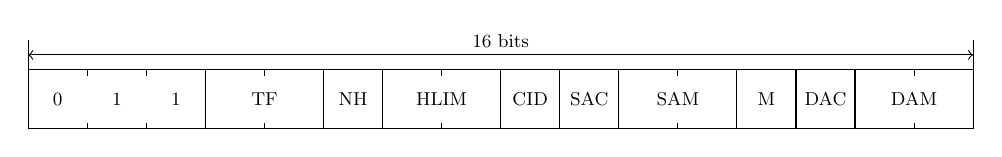
\begin{tikzpicture}[scale=0.75, every node/.append style={scale=0.75}]
		\draw (0,0) rectangle (16,1);
		\draw (0,1) -- ++(0,0.5);
		\draw (16,1) -- ++(0,0.5);
		\draw[<->] (0,1.25) -- (16,1.25) node[midway, above] {\small 16 bits};

		\foreach \x in {1,2,...,15}{
			\draw (\x,1) -- ++(0,-0.1);
			\draw (\x,0) -- ++(0,0.1);
		}

		\draw (3,0) -- ++(0,1);
		\node at (0.5, 0.5) {\small 0};
		\node at (1.5, 0.5) {\small 1};
		\node at (2.5, 0.5) {\small 1};

		\draw (5,0) -- ++(0,1);
		\node at (4, 0.5) {\small TF};

		\draw (6,0) -- ++(0,1);
		\node at (5.5, 0.5) {\small NH};

		\draw (8,0) -- ++(0,1);
		\node at (7, 0.5) {\small HLIM};

		\draw (9,0) -- ++(0,1);
		\node at (8.5, 0.5) {\small CID};

		\draw (10,0) -- ++(0,1);
		\node at (9.5, 0.5) {\small SAC};

		\draw (12,0) -- ++(0,1);
		\node at (11, 0.5) {\small SAM};

		\draw (13,0) -- ++(0,1);
		\node at (12.5, 0.5) {\small M};

		\draw (14,0) -- ++(0,1);
		\node at (13.5, 0.5) {\small DAC};

		\node at (15, 0.5) {\small DAM};

	\end{tikzpicture}
	\end{center}
	\caption{IPHC Format}
	\label{fig:6lo_iphc}
\end{figure}